\section{Dependent Type String Indexing is a Monoid}\label{sec:monoid}



\subsection{String Matching Definition}

We define the String Matching data type
@SM target@ to contain a string field @input@ and
a list of all the indices on @input@ where the
@target@ appears.
%
\begin{code}
data SM (target :: Symbol) where
  SM :: input:RString
     -> indices:[GoodIndex input target]
     -> SM target
\end{code}
%
We used type literals to parameterize the type over
the Symbol @target@.
%
This encoding is required to allow definition of
an identity element, as explained later~(\S~\ref{subsec:monoid:methods}).
%
The input field, of type @RString@, is a refined wrapper on
a String manipulation library that
1. allows for constant time string indexing, and
2. provides various string lemmata.
%
The library @RString.hs@~\footnote{
\href{https://github.com/nikivazou/verified_string_indexing/blob/master/src/String.hs}
     {\url{https://github.com/nikivazou/verified_string_indexing/blob/master/src/String.hs}}}
implements @RString@ as @ByteStrings@,
and \textbf{assumes} various String properties,
like left identity:
\begin{code}
assume leftIdentity :: s:RSTring -> { s <+> stringMempty == s }
\end{code}
%
The indices field is a list of good indices.
%
For simplicity we are using Haskell's built in lists but in the
implementation we use a user defined reflected list data type similar
to that presented in section~\ref{sec:haskell-proofs}.
%
A @GoodIndex input target@ is a refined type alias
for an integer @i@ that
1. is a natural number,
2. @target@ is a substring of @input@ appearing at position @i@.
%
\begin{code}
type GoodIndex Input Target
  = {i:Nat | isGoodIndex Input (fromString Target) i }

isGoodIndex :: RSTring -> RSTring -> Int -> Bool
isGoodIndex input target i
  =  (subString input i (stringLen target)  == target)
  && (i + stringLen target <= stringLen input)
\end{code}
%

As an example, the good indices of @"abcab"@ on @"ababcabcab"@
are @[2,5]@ while any other index is bad.
\begin{code}
goodSM :: SM "abcab"
goodSM = SM "ababcabcab" [2, 5]

badSM  :: SM "abcab"
badSM  = SM "ababcabcab" [0, 7]
\end{code}
\NV{Liquid Haskell actually will reject both the above, as the stringLen and subString functions are uninterpreted}

\subsection{Monoid Laws}
In the rest of this section we will prove that
the String Matching structure is a Monoid.
%
A structure @m@ is a monoid,
there is an identity element @mempty :: a@
and an associative appending function @(<>) :: a -> a -> a@.
That is, @mempty@ and @(<>)@ should satisfy the following laws
\begin{figure}
\begin{code}
idLeft :: x:a -> {x <> mempty == x }
idRight:: x:a -> {mempty <> x == x }
assoc  :: x:a -> y:a -> z:a -> {(x <> y) <> z == x <> (y <> z)}
\end{code}
\caption{Monoid Laws}
\label{fig:monoid:laws}
\end{figure}
%
To prove that the String Matching operator @SM@
is a monoid, we use the fact that the String and list
of indices contained in its fields are also monoids.
%
Figure~\ref{fig:monoids} defines the monoid operators used
in this section.
%
\begin{figure}
$$
\begin{array}{c c c c }
\text{Structure} & \text{Identity} & \text{Mappend} & \text{Laws} \\
\hline
\texttt{List} & \listMempty & (\listMappend) & \text{PROVEN} \\
\texttt{SM} & \mempty & (\mappend) & \text{PROVEN} \\
\texttt{RString} & \stringMempty & (\stringMappend) & \text{ASSUMED}
\end{array}
$$
\caption{Monoid Structures}
\label{fig:monoids}
\end{figure}


\subsection{Monoid Methods for String Matching}~\label{subsec:monoid:methods}
Next, we define the mappend and identity elements for string matching.
We reflect the definitions into logic, to latter use them to prove
the monoid laws.

The \textit{identity element} of @SM t@, for each target @t@, is
defined to contain the identity @RString@ (@stringMempty@) and the
identity @List@ (@listMempty@).
\begin{code}
reflect mempty
mempty:: forall (t :: Symbol). SM t
mempty = SM stringMempty listMempty
\end{code}
%
Note, that if target was encoded as a value argument, instead of a
type parameter, then there would be no way to define an identity
element for each expression argument.
%
\JP{I think the type parameter is more necessary to define mappend}


The @(mappend)@ operator,
mappends the two input strings.
The appended indices, as depicted in Figure~\ref{fig:mappend:indices},
are the concatenations of three list indices:
\begin{enumerate}
\item The indices @is1@ from the first input, casted to be good indices in the new structure,
\item the new indices @newIs@ created when concatenating the two strings, and
\item the indices @is2@ from the second input, shifted right @stringLen i2@ points.
\end{enumerate}
%
\begin{figure}
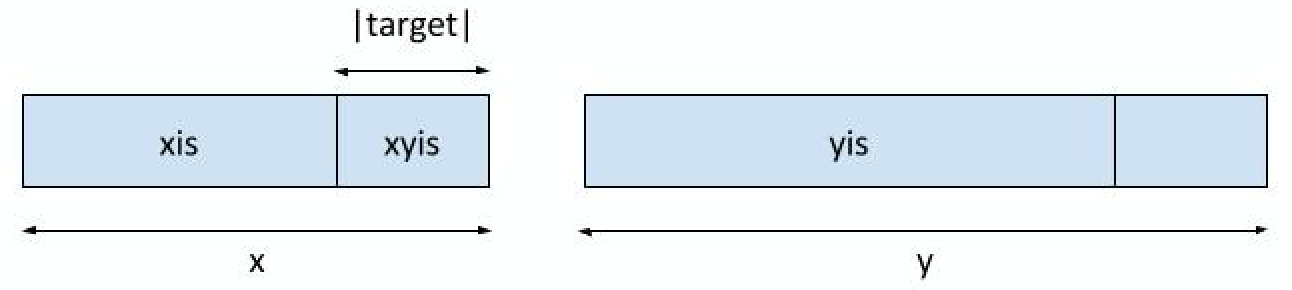
\includegraphics[scale=0.5]{makeIndices}
\caption{Mappend indices of String Matcher}
\label{fig:mappend:indices}
\end{figure}
%
The above are summarized in the Haskell definition of @(<>)@
\begin{code}
reflect mappend
(mappend)::forall (t::Symbol). KnownSymbol t => SM t -> SM t -> SM t
(SM i1 is1) mappend (SM i2 is2)
  = SM (i1 stringMappend i2) (is1' listMappend newIs listMappend is2')
  where
    tg    = fromString (symbolVal (Proxy :: Proxy t))
    is1'  = map (castGoodIndexLeft tg i1 i2) is1
    newIs = makeNewIndices i1 i2 tg
    is2'  = map (shiftStringRight tg i1 i2) is2
\end{code}

\paragraph{Step 1: Casting Good Indices}
If @is@ is a list of good indices for string @i1@ with respect to a target @tg@,
then @is@ is a list of good indices for the string @i1 stringMappend i2@, for each @i2@
for the same target.
%
To establish the above property,
we need the property from refined string
that states that
for each string @input@ and @input'@
and each integers @i@ and @j@ whose sum does not exceed the length of @input@,
the @subString@ on @input@ from @i@ with length @j@
is equal to
the @subString@ on @input stringMappend input'@ from @i@ with length @j@:
%
\begin{code}
subStringConcatLeft
    :: sl:RString -> sr:RString -> j:Int
    ->  i:{Int | i + j <= stringLen sl }
    ->  { subString sl i j == subString (sl stringMappend sr) i j }
\end{code}
%
To cast an index list of good indices in the above way,
we cast the above property to every element of the list
%
\begin{code}
reflect castGoodIndexRightList
castGoodIndexLeft
  :: tg:RString -> sl:RString -> sr:RString
  -> i:GoodIndex sl tg
  -> {v:GoodIndex (sl stringMappend sr target | v == i}

castGoodIndexLeft tg sl sr i
  = cast (subStringConcatLeft sl sr (stringLen tg) i) i
\end{code}
%
Where @cast p x@
returns @x@, after enforcing the properties of @p@ in the logic
\begin{code}
cast :: b -> x:a -> {v:a | v == x }
cast _ x = x
\end{code}
%
Moreover, the translation of @cast p x@ into the logic, is merely @x@
thus allowing random (\ie non-reflected) Haskell expressions appearing in @p@.

\paragraph{Step 2: Creation of new indices}
When concatenating two new string inputs @i1@ and @i2@,
the @stringLen tg@ last positions of @i1@ combined with the initial part of @i2@
may form new good indices.
%
@makeNewIndices s1 s2 target@ creates all such good new indices.
%
If the length of the @target@ is less than 2, then no new good indices are creates,
thus the function returns the empty list.
Otherwise, we search @concatString s1 s2@ for substring of @target@
in the range @[maxInt (stringLen s1 - (stringLen target-1)) 0, stringLen s1 - 1]@
\begin{code}
reflect makeNewIndices
makeNewIndices
  :: s1:RString -> s2:RString -> target:RString
  -> [GoodIndex {s1 stringMappend s2} target]
makeNewIndices s1 s2 target
  | lenStr target < 2
  = []
  | otherwise
  = makeIndices (s1 stringMappend s2) target lo hi
  where
    lo = maxInt (lenStr s1 - (lenStr target-1)) 0
    hi = lenStr s1 - 1
\end{code}
%
@makeIndices input target lo hi@
recursively searches for good indices on @input@ with respect to @target@
from @lo@ to @hi@.
%
\begin{code}
reflect makeIndices
makeIndices
  :: input:RString -> target:RString -> lo:Nat
  -> hi:Int -> [GoodIndex input target]
  / [hi - lo]
makeIndices input target lo hi
  | hi < lo
  = N
makeIndices input target lo hi
  | isGoodIndex input target lo
  = lo `C` rest
  | otherwise
  = rest
  where
    rest = makeIndices input target (lo + 1) hi
\end{code}
%
The notation @[hi-lo]@ declares that @makeIndices@ terminates, as the metric @hi - lo@
is a non-negative values that decreases at each recursive call.

\paragraph{Note on complexity.}
Given that the implementation of @RString@
allows substring checking via indexing, that is in constant time,
then @makeNewIndices@ and thus @(<>)@ requires @lenStr target@ checks,
that is constant checks with respect to the string input.

\paragraph{Step 3: Shift Good Indices}
If @is@ is a list of good indices for string @i2@ with respect to a target @tg@,
to get a list of good indices for the string @i1 stringMappend i2@,
we need to shift each element of @is@ @stringLen i1@ right.
%
Moreover, to persuade Liquid Haskell that the shifted indices are good indices
we need to apply the refined string theorem that states
for each string @sl@ and @sr@
and each integers @i@ and @j@,
the @subString@ on @sr@ from @i@ with length @j@
is equal to
the @subString@ on @sl stringMappend sr@ from @stringLen sl + i@ with length @j@:
%
\begin{code}
assume subStringConcatRight
  :: sl:RString -> sr:RString
  -> j:Int -> i:Int
  -> {subStr sr i j == subStr (sl stringMappend sr) (lenStr sl+i) j}
\end{code}

Thus, @shiftStringRight@ both appropriately shifts the index
and casts the shifted index using the above theorem:
\begin{code}
shiftStringRight
  :: tg:RString -> sl:RString -> sr:RString
  -> i:GoodIndex sr tg
  -> {v:(GoodIndex (sl stringMappend sr) tg) | v == i + lenStr sl}
shiftStringRight tg sl sr i
  = subStringConcatRight sl sr (stringLen tg) i)
     `cast` shift (stringLen sl) i
\end{code}


\subsection{String Matching is a Monoid}
We conclude this section by proving
that the @mempty@ and @(mappend)@
operators we defined satisfy the monoid laws.
%
In the prove, we express
\begin{itemize}
\item the monoid laws as liquid types, and
\item the monoid proofs as Haskell functions.
\end{itemize}
Then, Liquid Haskell checks that the functions indeed check the corresponding laws.

\begin{theorem}\label{theorem:monoid}
String Matching is a Monoid for the operations @mempty@ and @(mappend)@.
\end{theorem}

\begin{proof}
Based on the Monoid Definition~\ref{definition:monoid},
to prove that string maching is a monoid, we need to prove that
there exist safe implementations of the monoid laws functions.
%
We implemented the monoid laws functions
and used Liquid Haskell to (machine) check correctness of our proof.

First, we prove \textit{left identity}
\begin{code}
idLeft :: x:SM t -> {x mappend mempty == x }
idLeft (SM i is)
  =  (SM i is) mappend (mempty :: SM t)
  ==. (SM i is) mappend (SM stringMempty listMempty)
  ==. SM (i stringMappend stringMempty) (is1 listMappend isNew listMappend is2)
      ? idLeftString i
  ==. SM i (is listMappend N listMappend N)
      ? (mapCastId tg i stringMempty is &&& newIsNullLeft i tg)
  ==. SM i is
      ? idLeftList is
  ***  QED
  where
    tg    = fromString (symbolVal (Proxy :: Proxy t))
    is1   = map (castGoodIndexRight tg i stringEmp) is
    isNew = makeNewIndices i stringEmp tg
    is2   = map (shiftStringRight tg i stringEmp) N
\end{code}
The proof proceeds by rewriting and using four lemmata
\begin{itemize}
\item Left Identity on lists, that is proven by structural induction.
\begin{code}
idLeftList :: x:[a] -> {x listMappend listMempty == x}
\end{code}
\item Left Identity on strings is provided by the string library that we trust.
\begin{code}
idLeftString :: x:RString -> {x stringMappend stringMempty == x}
\end{code}
\item Identity of casting is proven by induction and identity on casts
\begin{code}
mapCastId :: tg:RString -> x:RString -> y:RString
  -> is:[GoodIndex x tg] ->
  -> {map (castGoodIndexRight tg x y) is == is}
\end{code}
\item No new indices are created by mappend
\begin{code}
newIsNullLeft :: s:RString -> t:RString
  -> {makeNewIndices s stringMempty t == listMempty }
\end{code}
The proof procceds by case splitting
on comparison of the lengths of @s@ and @t@.
At each case we prove by induction that all
the potential new indices will be out of bounds and thus
no new good indices can be created.
\end{itemize}

\NV{Actually, the right identity proof is simpler, maybe put it first}

- The proof of \textit{right identity} is similar
\begin{code}
idRight :: x:SM t -> {mempty mappend x == xs }
idRight (SM i is)
  =  (mempty :: SM t) mappend (SM i is)
  ==. (SM stringMempty listMempty) mappend (SM i is)
  ==. SM (stringMempty <+> i) (is1 ++ isNew ++ is2)
       ? idRightString i
  ==. SM i (N ++ N ++ is)
       ? (mapShiftZero tg i is &&& newIsNullRight i tg)
  ==. SM i is
       ? idRightList is
  *** QED
  where
    tg    = fromString (symbolVal (Proxy :: Proxy t))
    is1   = map (castGoodIndexRight tg i stringEmp) N
    isNew = makeNewIndices stringEmp i tg
    is2   = (map (shiftStringRight tg stringEmp i) is)
\end{code}
The proof uses again four lemmata.
\begin{itemize}
\item Right Identity on lists, that is proven by structural induction.
\begin{code}
idRightList :: x:[a] -> {listMemtpy listMappend x == x}
\end{code}
\item Right Identity on strings is provided by the string library that we trust.
\begin{code}
idRightString :: x:RString -> {stringMemepty stringMappend x == x}
\end{code}
\item Identity of shifting by an empty string is proven by induction and
the assumption that empty string has length 0
\begin{code}
mapShiftZero :: tg:RString -> i:RString -> is:[GoodIndex i target]
  -> {map (shiftStringRight tg stringMempty i) is == is }
\end{code}
\item No new indices are created by mappend
\begin{code}
newIsNullLeft :: s:RString -> t:RString
  -> {makeNewIndices stringMempty s t == listMempty }
\end{code}
The proofs relies on the fact that @makeIndices@
will be called on the range @[0, -1]@ and immediately return @listMemepty@.
\end{itemize}
- Finally we prove \textit{associativity}.
For space, we omit the detailed proof, and only give the interesting steps.
In the proof we need to show equality of two string matchers,
thus we need to show that their input and induces fields are respectively equal.
%
Equality of the input fields follows by associativity of RStrings.
%
The proof of index equlity proceeds in three steps.

\begin{enumerate}
\item Firstly, using list associativity and distribution of index shifting,
we group the indices in the five lists shown in Figure~\ref{fig:mappend:assoc}.
The indices of the input @x@,
the new indices from mappending @x@ to @y@,
the indices of the input @y@,
the new indices from mappending @x@ to @y@, and
the indices of the input @z@.
\item The representation of each group depends on the order of appending.
For example, if @zis1@ (resp. @zis2@) is the group @zis@ when
right (resp. left) mappend happened first, then we have
\begin{code}
zis1 = map (shiftStringRight tg xi (yi stringMappend zi))
       map (shiftStringRight tg yi zi) zis

zis2 = map (shiftStringRight tg (xi stringMappend yi) zi) zis
\end{code}
That is, in right first, the indices of @z@ are first shifted
by the length of @yi@ and then by the length of @xi@,
while in the left first case, the indices of @z@ are shifted by the
length of @xi stringMappend yi@.
In this second step of the proof, we prove using lemmata,
the equivalence of the group representation.
Equivalence of @xis@ and @zis@ is trivial,
but for the rest three groups, as we later discuss is more interesting,
as it depends on the relative lengths of the target and the input of @y@.
\item Finally, once we proved equivalence of representations,
we use again list associativity and distribution of casts to wrap the index groups
back in string matchers
\end{enumerate}
\begin{figure}
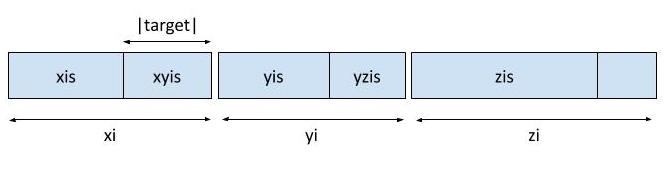
\includegraphics[scale=0.5]{AssociativeIndices}
\label{fig:mappend:assoc}
\end{figure}
Bellow we present the skeleton of the proof, while the detailed proof can be found online\footnote{\NV{GIVE PRoof link}}.
\begin{code}
assoc x@(SM xi xis) y@(SM yi yis) z@(SM zi zis)
  -- Step 1: unwrapping the indices
  =   x <> (y <> z)
  ==. (SM xi xis) <> ((SM yi yis) <> (SM zi zis))
                         ...
  -- via list associativity and distribution of shifts

  -- Step 3: Equivalence of representations
  ==. SM i (xis1 ++ ((xyis1 ++ yis1 ++ yzis1) ++ zis1))
  ==. SM i (xis1 ++ ((xyis1 ++ yis1 ++ yzis1) ++ zis1))
      ? castConcat tg xi yi zi xis
  ==. SM i (xis2 ++ ((xyis1 ++ yis1 ++ yzis1) ++ zis2))
      ? mapLenFusion tg xi yi zi zis
  ==. SM i (xis2 ++ ((xyis2 ++ yis2 ++ yzis2) ++ zis2))
      ? assocNewIndices y tg xi yi zi yis

  -- Step 3: Wrapping the indices
                         ...
  -- via list associativity and distribution of casts
  ==. (SM xi xis <> SM yi yis) <> SM zi zis
  =   (x <> y) <> z
  *** QED
  where
    yzis1 = map (shiftStringRight tg xi (yi <+> zi)) yzis
    yzis2 = makeNewIndices (xi <+> yi) zi tg

    yzis  = makeNewIndices yi zi tg

    i     = xi stringMappend (yi stringMappend zi)
\end{code}
Finally, we present the lemma @assocNewIndices@
that proofs equivalence of representation in the three
groups @xyis@, @yis@, and @yzis@.
The proof proceeds by case analysis in the relative size of
the target @tg@ and the middle input @yi@.
%
If the target is smaller than @yi@
then we can prove equivalence of each of the groups independently
via respective lemmata.
%
Otherwise, independent equivalence does not hold.
Thus, when @yi@ is smaller than the target,
the group @xyis1@ (similarly @yzis1@)
is not provably equal to @xyis2@ (similarly @yzis2@).
When @yi@ is smaller than the target,
when appending @x@ with @y mappend z@ new indices may occur because
of the suffix of @z@, these indices will not occur when appending @x@ with @y@.
%
Yet, the appending of the two new index groups are provably equal,
@xyis1 listMappend yzis1 == xyis2 listMappend yzis2@.
The lemma proof using append equivalence and the fact @yis1 == yis2 == []@
to conclude that the appending of all the three groups is always equivalent.

\begin{code}
-- proof that
-- xyis1 ++ yis1 ++ yzis1 == xyis2 ++ yis2 ++ yzis2
assocNewIndices y tg xi yi zi yis
  | stringLen tg <= stringLen yi
  =   xyisEquivalence xi yi zi tg
  &&&  yisEquivalence xi yi zi tg yis
  &&& yzisEquivalence xi yi zi tg
  | stringLen yi < stringLen tg
  =  xyis1 listMappend yis1 listMappend yzis1
  ==. xyis1 listMappend [] listMappend yzis1 ? emptyIndices y yis
  ==. xyis1 listMappend yzis1 ? idLeftList xyis1
  ==. xyis2 listMappend yzis2 ? shiftNewIndices xi yi zi tg
  ==. (xyis2 listMappend []) listMappend yzis2 ? idLeftList xyis2
  ==. (xyis2 listMappend yis2) listMappend yzis2 ? emptyIndices y yis
  *** QED
\end{code}


\qed\end{proof}
